\documentclass{standalone}
\usepackage{pgfplots}
\pgfplotsset{compat=1.8}

\begin{document}
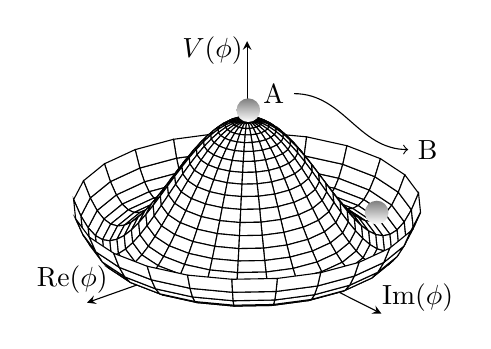
\begin{tikzpicture}
  \begin{axis}[
      axis lines=center,
      view={140}{25},
      axis equal,
      domain=0:360,
      y domain=0:1.25,
      xmax=1.5,ymax=1.5,zmin=0,zmax=1.5,
      x label style={at={(axis description cs:0.18,0.29)},anchor=north},
      y label style={at={(axis description cs:0.82,0.25)},anchor=north},
      z label style={at={(axis description cs:0.44,0.8)},anchor=north},
      xlabel = $\mathrm{Re}(\phi)$,
      ylabel=$\mathrm{Im}(\phi)$,
      zlabel=$V(\phi)$,
      ticks=none,
      clip bounding box=upper bound
    ]

    \addplot3 [surf, shader=flat, draw=black, fill=white, z buffer=sort] ({sin(x)*y}, {cos(x)*y}, {(y^2-1)^2});
  \end{axis}
  \shade (3.47,3.5) circle [radius=0.15cm];
  \shade (5.1,2.2) circle [radius=0.15cm];
  \node[anchor=east] at (4.05,3.71) (text) {A};
  \node[anchor=west] at (5.5,3.0) (description) {B};
  \draw (description) edge[out=180,in=0,<-] (text);
\end{tikzpicture}
\end{document}